\documentclass{../includes/TechDoc}
\usepackage[T1]{fontenc}
\usepackage[utf8]{inputenc}
\usepackage{hyperref}
\usepackage{amssymb}
\usepackage{amsmath,amsthm,mathtools}

\setcounter{tocdepth}{2}
\setcounter{secnumdepth}{3}

\title{Приложение для совместного просмотра фильмов}
\author{Студент группы БПИ194}{???}
\academicTeacher{Старший преподаватель департамента программной инженерии факультета компьютерных наук}{А. В. Поповкин}

\documentTitle{Техническое задание}
\documentCode{RU.17701729.02.07-01 ТЗ 01-1}

\begin{document}
    \maketitle

    \tableofcontents

    \section{Введение}

\subsection{Наименование программы}

\subsubsection{Наименование программы на русском языке}

Приложение для совместного просмотра фильмов.

\subsubsection{Наименование программы на английском языке}

Application for Collective Movie Watching.

\subsection{Краткая характеристика области применения}

Приложение предназначено для онлайн-просмотра видеофайлов с синхронизацией видеопотока между несколькими пользователями.


\section{Основания для разработки}

Приказ декана факультета компьютерных наук И.В. Аржанцева ``Об утверждении тем, руководителей курсовых работ студентов
образовательной программы <<Программная инженерия>> факультета компьютерных наук'' № XXX от XX.XX.XXXX.


    \section{Назначение разработки}

\subsection{Функциональное назначение}

Функциональным назначением программы является:
\begin{enumerate}
    \item показ онлайн-видеороликов:
    \begin{enumerate}
        \item загруженных пользователем в одном из поддерживаемых форматов;
        \item интегрированных через сторонние сервисы для просмотра видео (YouTube, VK, Rutube);
    \end{enumerate}
    \item синхронизация видеопотока между разными пользователями;
    \item обеспечение функционала по социальному взаимодействию пользователей:
    \begin{enumerate}
        \item обычный текстовый ввод сообщений;
        \item ввод сообщений посредством голоса с последующим переводом голоса в текстовый вид;
        \item отправка «реакций» в виде стикеров для быстрых эмоций.
    \end{enumerate}
\end{enumerate}


\subsection{Эксплуатационное назначение}

Программа может быть использована пользователями для просмотра фильмов со своими близкими на большом расстоянии.

    \section{Требования к программе}

\subsection{Требования к функциональным характеристикам}

Программа состоит из двух основных компонент: клиентской и серверной частей, между которыми должно быть налажено
взаимодействие.

\subsubsection{Требования к клиентской части}
Клиент должен иметь интерфейс, позволяющий пользователю взаимодействовать с программой с минимальной предварительной
подготовкой.
Дизайн интерфейса должен соответствовать современным тенденциям, обладать адаптивностью под различные характеристики
экранов.
Интерфейс должен менять свой стиль в зависимости от времени суток для имитации освещения в комнате.

Клиент реализует три основных экрана.
На каждом экране расположен свой набор элементов:\\

На главной странице:
\begin{enumerate}[noitemsep]
    \item Поле для ввода ссылки на сторонний видео-ресурс (YouTube, VK, Rutube).
    Поле должно быть «универсальным» для всех ресурсов.
    \item Поле для загрузки файла (.torrent или обычного видео-формата).
    \item Статистика: количество активных пользователей, количество запущенных комнат.
    \item Ссылки на социальные сети проекта;
    \item Кнопка доната, топ донатов за неделю, топ донатов за месяц.
\end{enumerate}

На странице комнаты:
\begin{enumerate}[noitemsep]
    \item Аккаунт пользователя.
    \item Ссылка для подключения к комнате.
    \item Список участников комнаты.
    \item Информация об обработке видео:
    \begin{enumerate}
        \item Процент загрузки;
        \item Процент обработки;
        \item Длительность;
        \item Максимальное качество.
    \end{enumerate}
    \item Дополнительные параметры для видео:
    \begin{enumerate}
        \item Возможность добавить аудиодорожку к видеофайлу;
        \item Возможность добавить субтитры к видеофайлу.
    \end{enumerate}
    \item Дополнительные параметры для комнаты:
    \begin{enumerate}
        \item Возможность добавить ещё одно видео в очередь просмотра;
        \item Настройка прав на добавление аудиодорожен:
        \begin{enumerate}
            \item только создатель;
            \item все пользователи;
            \item выбранные пользователи;
        \end{enumerate}
        \item Настройка прав на перемотку/остановку/возобновление видео:
        \begin{enumerate}
            \item только создатель;
            \item все пользователи;
            \item выбранные пользователи.
        \end{enumerate}
    \end{enumerate}
    \item Текстовый чат пользователей с возможностью его чтения и отправки сообщений.
    \item Проигрыватель с видео.
\end{enumerate}

В проигрывателе с видео:
\begin{enumerate}[noitemsep]
    \item Кнопка изменения качества видео.
    \item Возможность изменения аудиодорожки в процессе просмотра, если есть такая возможность.
    \item Возможность включения/отключения/изменения субтитров, если есть такая возможность.
    \item Возможность тремя способами отправлять сообщения в чат прямо из плеера, не выходя из полноэкранного режима:
    \begin{enumerate}
        \item Обычный текстовый ввод сообщений;
        \item Ввод сообщений посредством голоса с последующим переводом голоса в текстовый вид;
        \item Отправка «реакций» в виде стикеров для быстрых эмоций.
    \end{enumerate}
    \item Отображение сообщений чата прямо в плеере.
    Чат может содержать текстовые сообщения и «реакции».
\end{enumerate}

\newpage

\subsubsection{Требования к серверной части}
На серверной части должен быть реализован алгоритм по преобразованию единого видеоролика в набор видеороликов меньшей длительности
(сегментов).
Также требуется добавить конвертацию видеоролика в видеоролики с меньшим качеством (Рис.~\ref{ris:server_converting}).

Должно быть реализовано взаимодействие с базой данных для хранения данных о комнатах.

\begin{figure}[h]
    \centering
    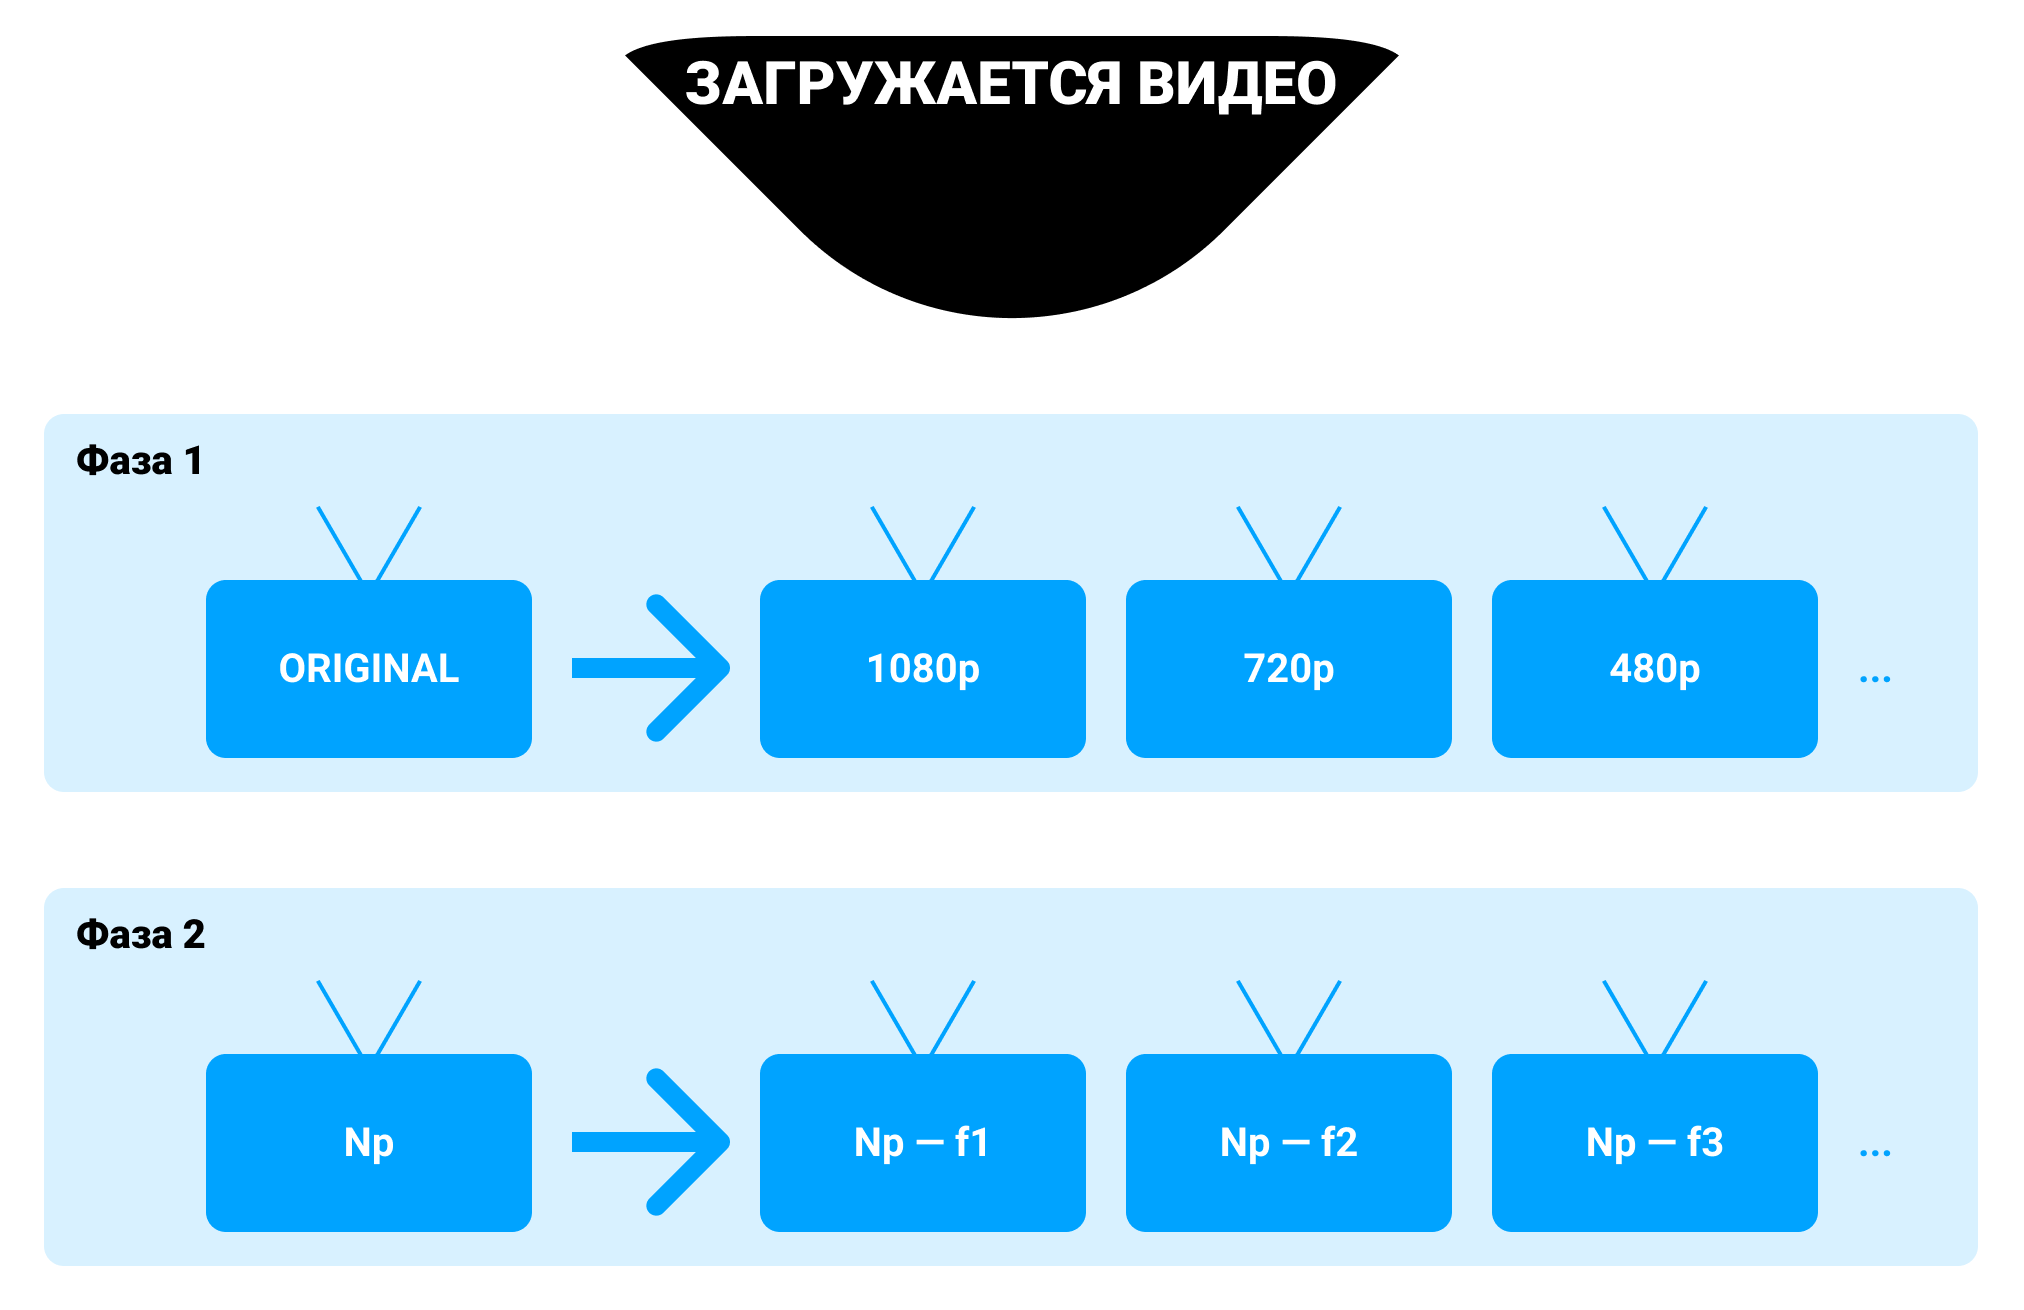
\includegraphics[width=1\linewidth]{images/server_converting.png}
    \caption{Алгоритм конвертации видео}
    \label{ris:server_converting}
\end{figure}

\newpage

\subsubsection{Требования к взаимодействию клиентской и серверной частей}
Взаимодействие между клиентом и сервером должно осуществляться посредством HTTP-запросов и WebSocket-подключений.

При получении HTTP-запроса (GET, POST, UPDATE, DELETE и т.д.) от клиента, сервер должен ответить сообщением в формате
JSON, содержащим необходимую информацию для работы клиента.

Для синхронизации видеопотока между разными клиентами используется протокол WebSocket.
В целях обеспечения наименьшей рассинхронизации видеопотока между клиентами, требуется хранить переменные \(diff\_sc\) и \(diff\_cs\) для
каждого клиента.
Данные переменные будут содержать в себе информацию о количестве затрачиваемого времени при передаче данных от сервера к клиенту или от клиента к серверу.

Формула для определения переменных \(diff\_sc\) и \(diff\_cs\): \begin{gather*}
                                                                    diff\_sc = time\_sc_2 - time\_sc_1\\
                                                                    diff\_cs = time\_cs_2 - time\_cs_1
\end{gather*}, где:
\begin{itemize}[noitemsep]
    \item[--] \(time\_sc_1\) — время отправки сообщения сервером;
    \item[--] \(time\_sc_2\) — время получения сообщения клиентом;
    \item[--] \(diff\_sc\) — разница между временем отправки и временем получения при передаче сообщения от сервера к клиенту;
    \item[--] \(time\_cs_1\) — время отправки сообщения клиентом;
    \item[--] \(time\_cs_2\) — время получения сообщения сервером;
    \item[--] \(diff\_cs\) — разница между временем отправки и временем получения при передаче сообщения от клиента к серверу.
\end{itemize}

Так как возможно подключение нескольких клиентов, требуется хранить содержимое значений \(diff\_sc_i\) и \(diff\_cs_i\) для всех \(n\) клиентов.

Алгоритм (Рис.~\ref{ris:interaction_format}) синхронизации видео единый:
\begin{enumerate}
    \item Клиент \(k\) отправляет серверу запрос на действие \(d\) (перемотку/приостановку/возобновление) видео.
    \item Сервер отправляет всем клиентам сообщение с текущим серверным временем.
    Клиенты принимают значение и считают разницу \(diff\_sc_i\) с учётом своего времени.
    Затем клиенты отправляют посчитанную разницу времени в миллисекундах обратно серверу, а также отправляют текущее клиентское время.
    С учётом полученной информации сервер считает разницу \(diff\_cs_i\).
    \item Сервер отправляет всем клиентам команду выполнить действие \(d\) и передаёт каждому клиенту задержку \(delay_i\),
    которая считается по формуле: \[ delay_i = \max(diff\_sc_1, \ldots, diff\_sc_n) - diff\_sc_i + diff\_cs_k, \;\;\; i \in [1, \ldots, n] \]
\end{enumerate}

Значение \(delay_i\) требуется по-разному использовать в различных ситуациях.
При организации совместного просмотра фильма возможны следующие сценарии:
\begin{itemize}
    \item[--] \textbf{Перемотка} видео на позицию \(t\) мс одним из клиентов.

    При получении такой команды все клиенты (кроме клиента-инициатора) выполняют перемотку видео на позицию \((t + delay_i)\) мс.
    \item[--] \textbf{Приостановка} видео одним из клиентов.

    При получении такой команды все клиенты (кроме клиента-инициатора) выполняют перемотку видео на \(delay_i\) мс назад.
    \item[--] \textbf{Возобновление} видео одним из клиентов.

    При получении такой команды все клиенты (кроме клиента-инициатора) выполняют перемотку видео на \(delay_i\) мс вперёд.
\end{itemize}

\begin{figure}[h]
    \centering
    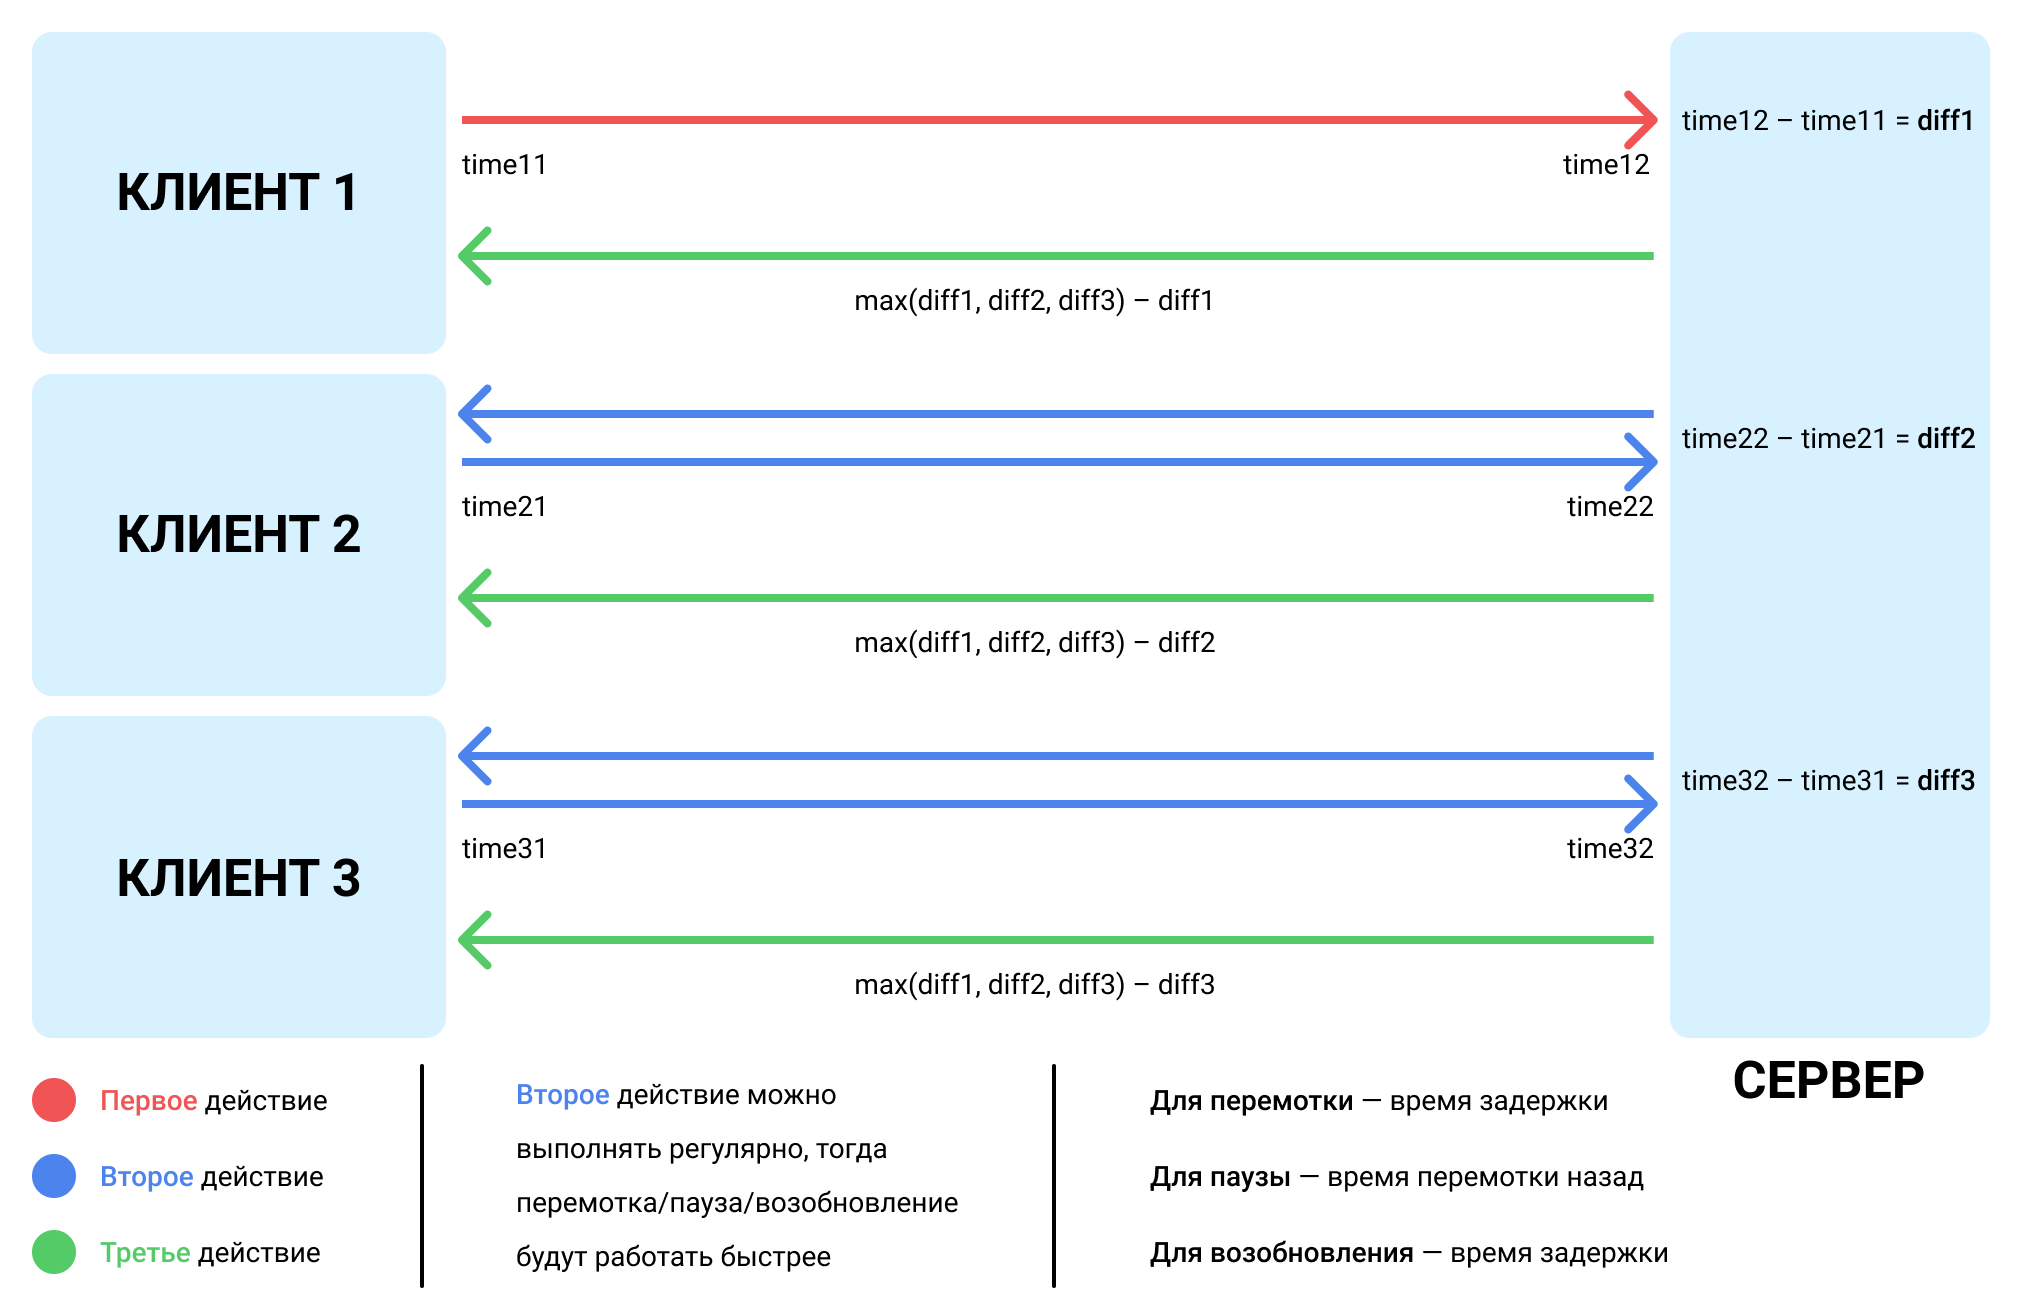
\includegraphics[width=1\linewidth]{images/interaction_format.png}
    \caption{Алгоритм синхронизации видеопотока}
    \label{ris:interaction_format}
\end{figure}

\newpage

\subsubsection{Требования к организации входных данных}
Входные данные программы должны быть организованы в виде вводимого в специальную форму текста или файла,
соответствеющего определённому шаблону.
Данные, вводимые вручную, проверяются на корректность после попытки сохранения;
данные, вводимые из файла, проверяются в ходе анализа и размещения данных.

\subsubsection{Требования к организации выходных данных}
Выходные данные программы должны быть организованы в виде визуальных эффектов интерфейса, текстов, картинок и
видеороликов, расположенных на WEB-странице.

Видеоролики должны делиться на фрагменты, которые в последствии WEB-проигрыватель должен склеивать в полноценное видео.

\subsection{Требования к надёжности}

\subsubsection{Требования к обеспечению надёжного (устойчивого) функционирования программы}

\paragraph{Требования для WEB-клиента}
Разрабатываемое приложение должно:
\begin{enumerate}
    \item не завершаться аварийно при возникающих ошибках.
\end{enumerate}

\paragraph{Требования для сервера}
Разрабатываемый сервер должен:
\begin{enumerate}
    \item запрещать доступ к REST API методам для неавторизованных пользователей;
    \item не показывать информацию из посторонних общежитий для авторизованных пользователей;
    \item не показывать чужие обращения пользователю;
    \item быть устойчивым к атакам следующего типа:
    \begin{enumerate}
        \item Cross-Site Scripting (XSS),
        \item SQL Injection,
        \item Local File Inclusion (LFI),
        \item Distributed Denial of Service (DDoS).
    \end{enumerate}
\end{enumerate}

\subsubsection{Время восстановления после отказа}
Время восстановления после отказа, вызванного сбоем электропитания технических средств (иными внешними факторами),
не фатальным сбоем (не крахом) операционной системы, не должно превышать времени, необходимого на перезагрузку
операционной системы и запуск программы, при условии соблюдения условий эксплуатации технических и программных средств.

Время восстановления после отказа, вызванного неисправностью технических средств, фатальным сбоем (крахом) операционной
системы, не должно превышать времени, требуемого на переустановку программных средств.

\subsubsection{Отказы из-за некорректных действий оператора}
Во избежание возникновения отказов программы по причине некорректных действий оператора следует обеспечить работу
конечного пользователя без предоставления ему административных привилегий.

\subsection{Условия эксплуатации}

\subsubsection{Климатические условия}

Климатические условия сопадают с климатическими условиями эксплуатации устройства.

\subsubsection{Требования к пользователю}

Пользователь должен обладать базовыми навыками работы с одной из операционных систем: Windows, macOS, Linux, Android,
iOS, а также с одним из браузеров: Google Chrome, Firefox, Safari, Microsoft Edge.

\subsection{Требования к составу и параметрам технических средств}

\subsubsection{Требования для WEB-клиента}
В состав технических средств может входить портативный компьютер или мобильный телефон.
Для корректной загрузки видеофайлов требуется стабильное интернет-подключение.

\subsubsection{Требования для сервера}
В состав технических средств должен входить компьютер или система компьютеров.
Допускается использование облачных сервисов.

\subsection{Требования к информационной и программной совместимости}

\subsubsection{Требования к программной совместимости}
Для корректной работы WEB-клиента должен использоваться один из следующих браузеров:
\begin{enumerate}[noitemsep]
    \item Google Chrome (86.0.4240.183+);
    \item Firefox (20.1+);
    \item Safari (14.0+);
    \item Microsoft Edge (86.0.622.63+).
\end{enumerate}

\subsubsection{Требования к исходным кодам и языкам программирования}

Исходные коды для WEB-клиента должны быть реализованы с использованием следующих языков и технологий:
\begin{enumerate}[noitemsep]
    \item HTML5 и CSS — для реализации графического представления клиента;
    \item JavaScript — для добавления динамики графическому интерфейсу;
    \item ReactJS или vue.js — для реализации архитектуры и программной логики WEB-клиента.
\end{enumerate}

Исходные коды для сервера должны быть реализованы с использованием следующих языков и технологий:
\begin{enumerate}[noitemsep]
    \item Java;
    \item Spring Boot — для реализации базовой архитектуры сервера;
    \item Spring Web — для реализации REST API методов и панели администрирования;
    \item Spring Thymeleaf — для миграций и версионирования базы данных;
    \item Hibernate — для работы с базой данных, для связки таблиц базы данных с классами Java;
    \item ffmpeg — для обработки видеофайлов: нарезка и изменение качества;
    \item PostgreSQL — использовать в качестве СУБД.
\end{enumerate}

\paragraph{Требования к взаимодействию клиентов с сервером}
Взаимодействие между WEB-клиентом и сервером должно происходить посредством HTTP-запросов и WebSocket-подключений.
При получении HTTP-запроса (GET, POST, UPDATE, DELETE и т.д.) от клиента, сервер должен ответить сообщением в формате
JSON, содержащим необходимую информацию для работы клиента.

\subsection{Требования к составу сетевых средств}

У устройства должен быть доступ к сети интернет для корректной работы WEB-клиента.

\subsection{Требования к маркировке и упаковке}

Сервер должен быть удалённо развёрнут на одном из облачных сервисов.
Для обеспечения переносимости требуется настроить контейнер Docker.

WEB-клиент публикуется на удалённом сервере с настроенным доменом «comnata.tv».

    \section{Требования к программной документации}

\subsection{Состав программной документации}

В состав программной документации должны входить следующие компоненты:
\begin{enumerate}
    \item Техническое задание (ГОСТ 19.201-78)
    \item Программа и методика испытаний (ГОСТ 19.301-78)
    \item Пояснительная записка (ГОСТ 19.404-79)
    \item Руководство оператора (ГОСТ 19.505-79)
    \item Текст программы (ГОСТ 19.401-78)
\end{enumerate}


\subsection{Специальные требования к программной документации}

Документы к программе должны быть выполнены в соответствии с ГОСТ 19.106-78 и ГОСТами к каждому виду документа (см. п. 5.1.);

Пояснительная записка должна быть загружена в систему Антиплагиат через LMS «НИУ ВШЭ».

Документация и программа сдаются в электронном виде в формате .pdf или .docx. в архиве формата .zip или .rar;

За один день до защиты комиссии все материалы курсового проекта:
\begin{itemize}
    \item[--] техническая документация,
    \item[--] программный проект,
    \item[--] исполняемый файл,
    \item[--] отзыв руководителя,
    \item[--] лист Антиплагиата
\end{itemize}
должны быть загружены одним или несколькими архивами в проект дисциплины «Курсовой проект 2019-2020» в личном кабинете в информационной образовательной среде LMS (Learning Management System) НИУ ВШЭ.


    \section{Технико-экономические показатели}

\subsection{Предполагаемая потребность}

Приложение может быть использовано пользователями, которые желают совместно с другими пользователями посмотреть видео и
фильмы, но не имеют возможности встретиться для этого лично.

\subsection{Экономические преимущества разработки по сравнению с отечественными и зарубежными аналогами}

На момент начала разработки на рынке были выявлены следующие аналоги:
\begin{itemize}
    \item[--] «\href{https://notalone.tv/}{vmeste.tv}».
    123123.
    \item[--] «NotAlone» (\href{https://notalone.tv/}{notalone.tv}).
    12123123.
    \item[--] «Facebook Messenger».
    233123.
\end{itemize}

    \section{Стадии и этапы разработки}

\subsection{Стадии и этапы разработки}

\begin{enumerate}
    \item техническое задание:
    \begin{enumerate}
        \item этапы разработки:
        \begin{enumerate}
            \item обоснование необходимости разработки программы;
            \item постановка задачи;
            \item сбор исходных материалов;
            \item выбор и обоснование критериев эффективности и качества разрабатываемой программы;
            \item обоснование необходимости проведения научно-исследовательских работ;
        \end{enumerate}
        \item разработка и утверждение технического задания:
        \begin{enumerate}
            \item определение требований к программе;
            \item определение стадий, этапов и сроков разработки программы и документации на неё;
            \item согласование и утверждение технического задания;
        \end{enumerate}
    \end{enumerate}
    \item технический проект:
    \begin{enumerate}
        \item разработка технического проекта:
        \begin{enumerate}
            \item уточнение структуры входных и выходных данных;
            \item разработка алгоритма решения задачи;
            \item определение формы представления входных и выходных данных;
            \item разработка структуры программы;
            \item окончательное определение конфигурации технических средств.
        \end{enumerate}
        \item утверждение технического проекта:
        \begin{enumerate}
            \item разработка пояснительной записки;
            \item согласование и утверждение технического проекта.
        \end{enumerate}
    \end{enumerate}
    \item рабочий проект:
    \begin{enumerate}
        \item разработка программы:
        \begin{enumerate}
            \item программирование и отладка программы.
        \end{enumerate}
        \item разработка программной документации:
        \begin{enumerate}
            \item разработка программных документов в соответствии с требованиями гост 19.101-77.
        \end{enumerate}
        \item испытания программы:
        \begin{enumerate}
            \item разработка, согласование и утверждение порядка и методики испытаний;
            \item корректировка программы и программной документации по результатам испытаний.
        \end{enumerate}
    \end{enumerate}
    \item подготовка и передача программы:
    \begin{enumerate}
        \item утверждение даты защиты программного продукта;
        \item подготовка программы и программной документации для презентации и защиты;
        \item представление разработанного программного продукта руководителю и получение отзыва;
        \item загрузка Пояснительной записки в систему Антиплагиат через ЛМС НИУ ВШЭ;
        \item загрузка материалов курсового проекта (курсовой работы) в ЛМС, проект дисциплины «Курсовая работа 2019» (п. 5.2);
        \item защита программного продукта (курсового проекта) комиссии.
    \end{enumerate}
\end{enumerate}

\subsection{Сроки разработки и исполнители}
Разработка должна закончиться в мае 2021 года.\\

Исполнители:
\begin{itemize}
    \item[--] Панфилов Егор Павлович, студент группы БПИ194 факультета компьютерных наук НИУ ВШЭ.

    Разработчик WEB-клиента.
    \item[--] Анненков Владислав Алексеевич, студент группы БПИ194 факультета компьютерных наук НИУ ВШЭ.

    Разработчик сервера.
\end{itemize}

    \section{Порядок контроля и приёмки}

Проверка программного продукта, в том числе и на соответствие техническому заданию, осуществляется исполнителем вместе с заказчиком согласно <<Программе и методике испытаний>>, а также пункту 5.2.

Защита выполненного проекта осуществляется комиссии, состоящей из преподавателей департамента программной инженерии, в утверждённые приказом декана ФКН сроки.


    \registrationList
\end{document}
